\chapter{Analyse Walker Demo}
\label{sec:analyse}
Zusätzlich zu den maschinellen Lernkomponenten stellt Unity auch Demonstrationsumgebungen bereit, in denen verschiedene Lösungen für gängige Verstärkungslernprobleme implementiert sind. In der Walker-Demo wird ein physisch simulierter Charakter darauf trainiert, zu einem Zielwürfel zu laufen. Die Demo implementiert bereits einige grundlegende Steuerungsmechanismen, die erforderlich sind, um einen Charakter in einer Umgebung zu bewegen. Aus diesem Grund wird in dieser Arbeit die Walker-Demo als Basis für die Entwicklung genutzt. 

Im folgenden Kapitel wird daher die Walker-Demo analysiert, um in den weiteren Kapiteln darauf aufzubauen. Es wird untersucht, wie die Lernumgebung aufgebaut ist. Anschließend werden der Ablauf und die Komponenten für das verstärkende Lernen analysiert. Zum Abschluss werden das Trainingsergebnis und die Bewegungsabläufe der Demo analysiert.
\section{Lernumgebung}
Die Umgebung besteht aus einem quadratischen Spielfeld mit einem Boden und vier Wänden, die der Charakter nicht verlassen kann (siehe Abbildung \ref{fig:szene_demo}). Diese Begrenzungen dienen dazu, die Bewegung des Charakters zu kontrollieren und sicherzustellen, dass die Lernumgebung konsistent bleibt. Die Umgebung umfasst weiterhin den Läufer und das Ziel.

\begin{figure}[H]
  \centering  
  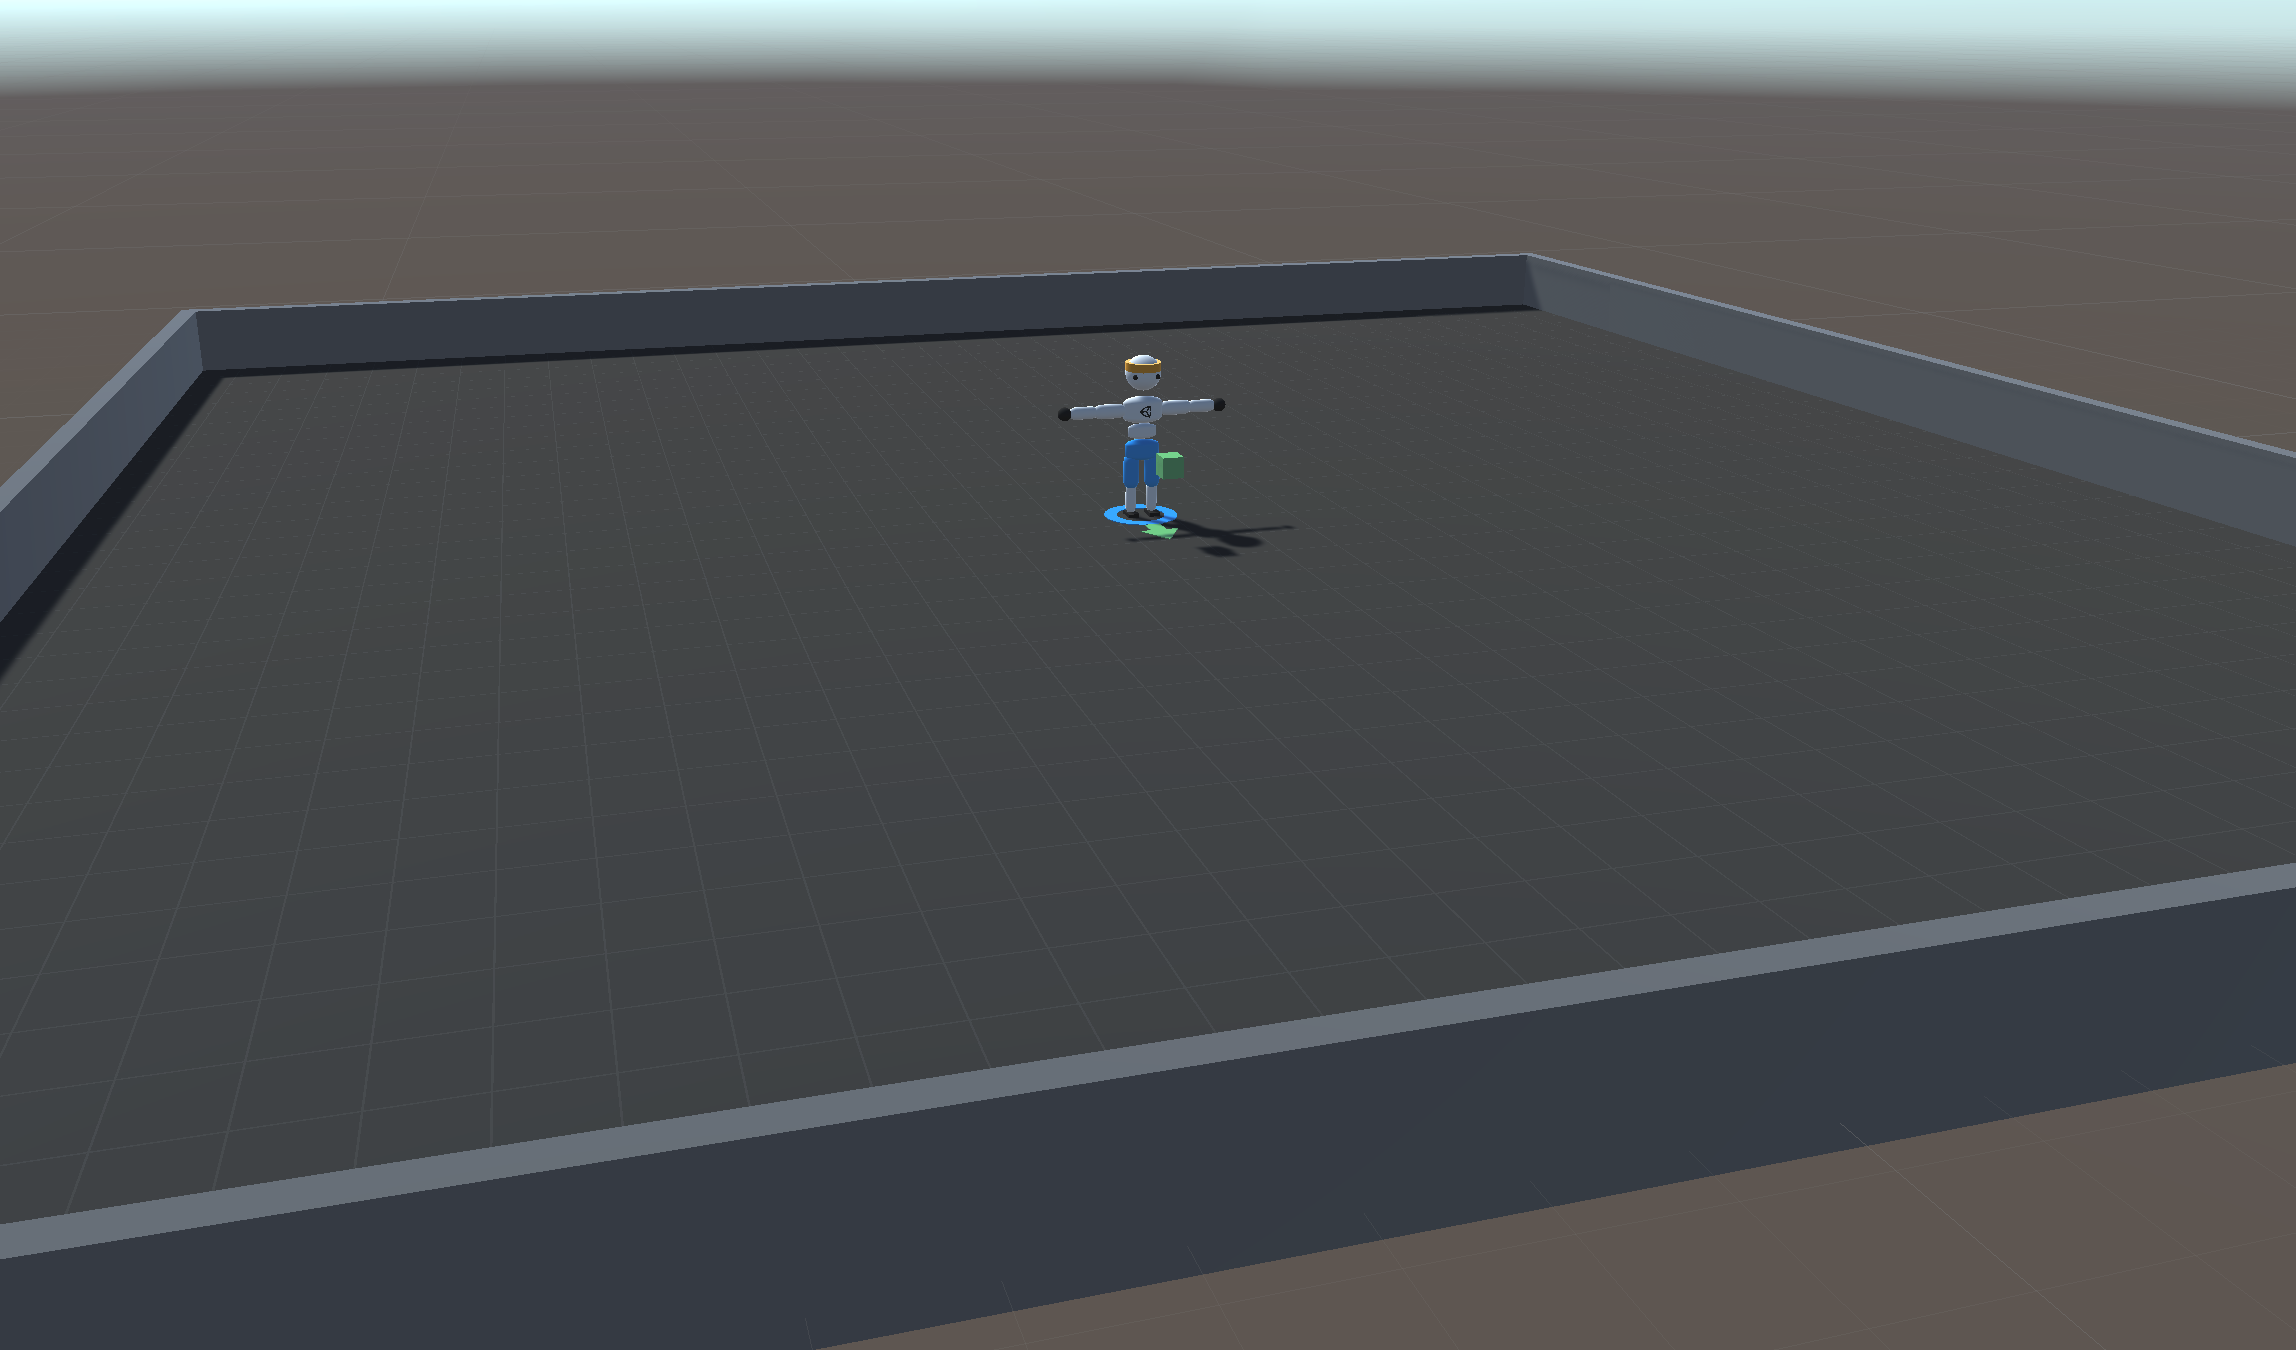
\includegraphics[width=0.8\textwidth]{img/szene_demo}
  \caption{Walker-Demo Umgebung}
  \label{fig:szene_demo}
\end{figure}

Der Läufer besteht aus einfachen geometrischen Körpern. Insgesamt 11 Kapseln, drei Kugeln und zwei Quadern, von welchen jede über eine Festkörper- und eine Kollisions-Physikkomponente verfügt. Die Gelenke zwischen den Körperteilen werden als Kugelgelenke simuliert, um eine flexible und natürliche Bewegung zu gewährleisten. Die genaue Physikkonfiguration der Körperteile wird in der Tabelle \ref{table:walker_körperteile} veranschaulicht. Diese Konfiguration spielt eine zentrale Rolle, da die gesetzten Freiheiten sowie Einschränkungen beeinflussen, wie der Läufer lernt, auf das Ziel zuzulaufen.

\begin{figure}[H]
  \centering  
  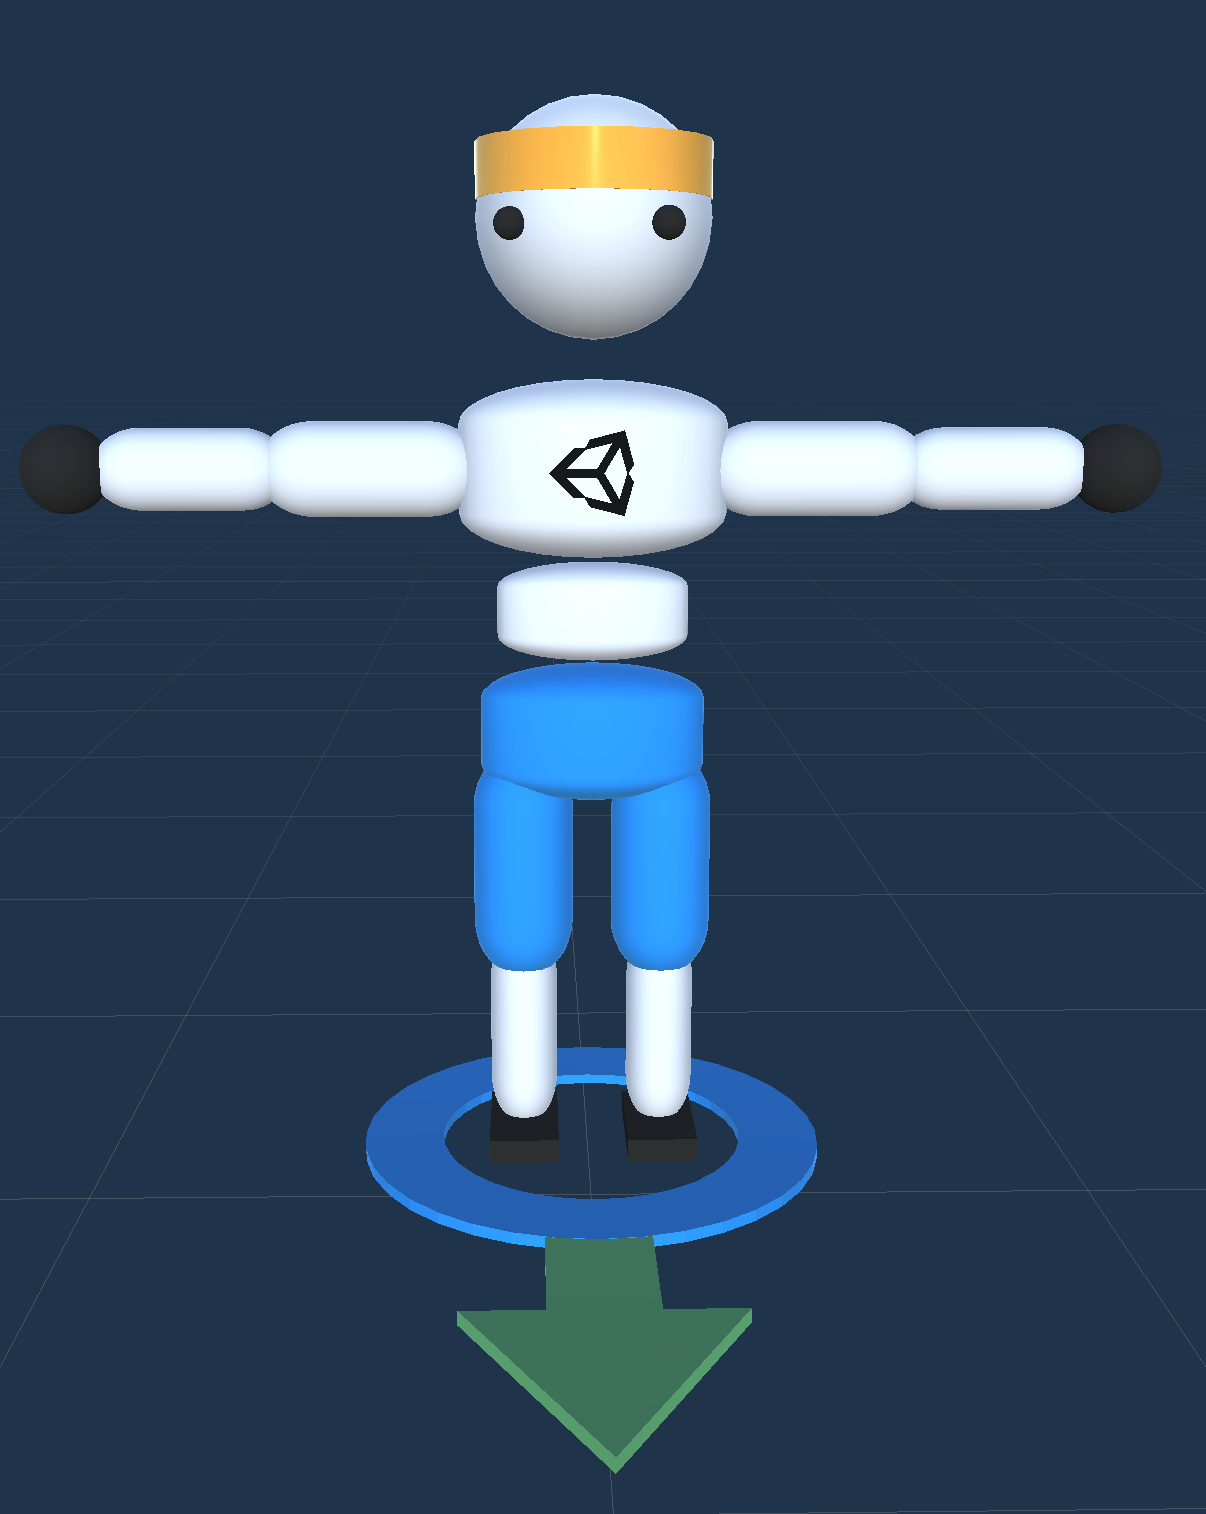
\includegraphics[scale=0.35]{img/charakter_walker}
  \caption{Walker-Demo Läufer}
  \label{fig:charakter_walker}
\end{figure}

\begin{table}[H]
  \centering
  {\rowcolors{1}{gray!10}{white}
  \begin{tabular}{ |p{3cm}|p{3cm}|p{2cm}|p{4cm}|p{2cm}| }
  \hline
  \textbf{Körpertei}l& \textbf{Verbundenes Körperteil} & \textbf{Gewicht} & \textbf{Winkellimits} & \textbf{Form} \\
  \hline
  Hüfte & - & 15kg & - & Kapsel \\
  \hline
  Wirbelsäule & Hüfte & 10kg & x(-20,20) y(-20,20) z(-15,15) & Kapsel \\
  \hline
  Oberkörper & Wirbelsäule & 8kg & x(-20,20) y(-20,20) z(-15,15) & Kapsel \\
  \hline
  Kopf & Oberkörper & 6kg & x(-30,10) y(-20,20) & Kugel \\
  \hline
  Oberarm LR & Oberkörper & je 4kg & x(-60,120) y(-100,100) & Kapsel \\
  \hline
  Unterarm LR & Oberarm & je 3kg & x(0,160) & Kapsel \\
  \hline
  Hand LR & Unterarm & je 2kg & - & Kugel \\
  \hline
  Oberschenkel LR & Hüfte & je 14kg& x(-90,60) y(-40,40) & Kapsel \\
  \hline
  Unterschenkel LR & Oberschenkel & je 7kg &  x(0,120) & Kapsel \\
  \hline
  Fuß LR & Unterschenkel & je 5kg & x(-20,20) y(-20,20) z(-20,20) & Quader \\
  \hline
  \end{tabular}}
  \caption{Walker Agent Körperteile}
  \label{table:walker_körperteile}
\end{table}

Das Walker Agent Skript definiert den Läufer als Agent für das maschinelle Lernen. In Abbildung \ref{fig:komponente_walker_agent} wird die Agentenkomponente im Inspektor gezeigt. Diese Komponente ist entscheidend für die Konfiguration des Läufers. Um die Komponente zu nutzen, müssen hier die Körperteile des Walkers referenziert werden. Das Walker Agent Skript registriert die Körperteile bei der Initialisierung in der Gelenk-Motor-Steuerung, wodurch eine effektive Schnittstelle zur Kontrolle der Gelenke geschaffen wird. Die Gelenk-Motor-Einstellungen (Joint Drive Settings) siehe Abbildung \ref{fig:komponente_joint_drive_controller} bestimmen die Stärke, mit welcher die Gelenke in die Zielstellung bewegt werden. Die Zielgeschwindigkeit kann manuell festgelegt werden oder während des Trainings in einem festgelegten Bereich variieren. Die Geschwindigkeit während des Trainings zu variieren hilft dem Agent sein Verhalten besser an Umgebungsveränderungen anzupassen. Als Letztes muss auch das Zielobjekt referenziert werden.

\begin{figure}[H]
  \centering  
  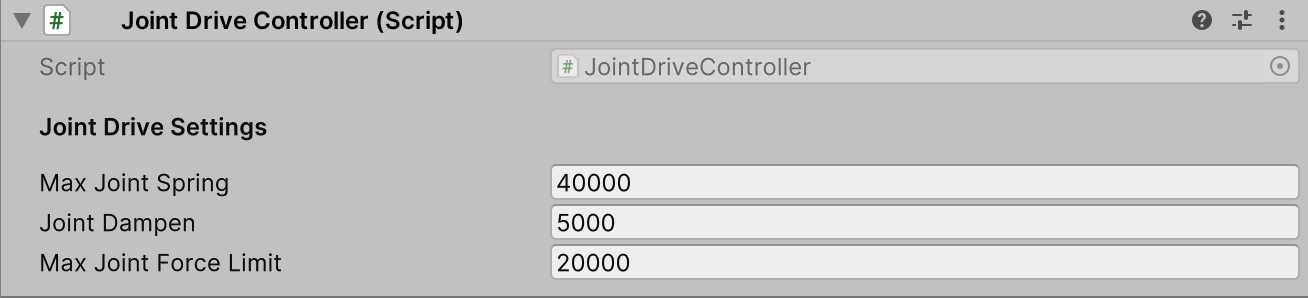
\includegraphics[width=0.8\textwidth]{img/komponente_joint_drive_controller}
  \caption{Gelenk Motor Steuerung}
  \label{fig:komponente_joint_drive_controller}
\end{figure}

\begin{itemize}
  \item Max Joint Spring: Bestimmt den Drehmoment, mit welchem das Gelenk in die Zielposition rotiert wird.
  \item Joint Dampen: Verringert den Drehmoment proportional zur Differenz zwischen aktueller Geschwindigkeit und der Zielgeschwindigkeit. Dadurch verringert es Schwingungen.
  \item Max Joint Force Limit: Gibt die maximale Kraft des Gelenks an (verhindert zu schnelle Bewegung bei großer Abweichung).
\end{itemize}

\begin{figure}[H]
  \centering  
  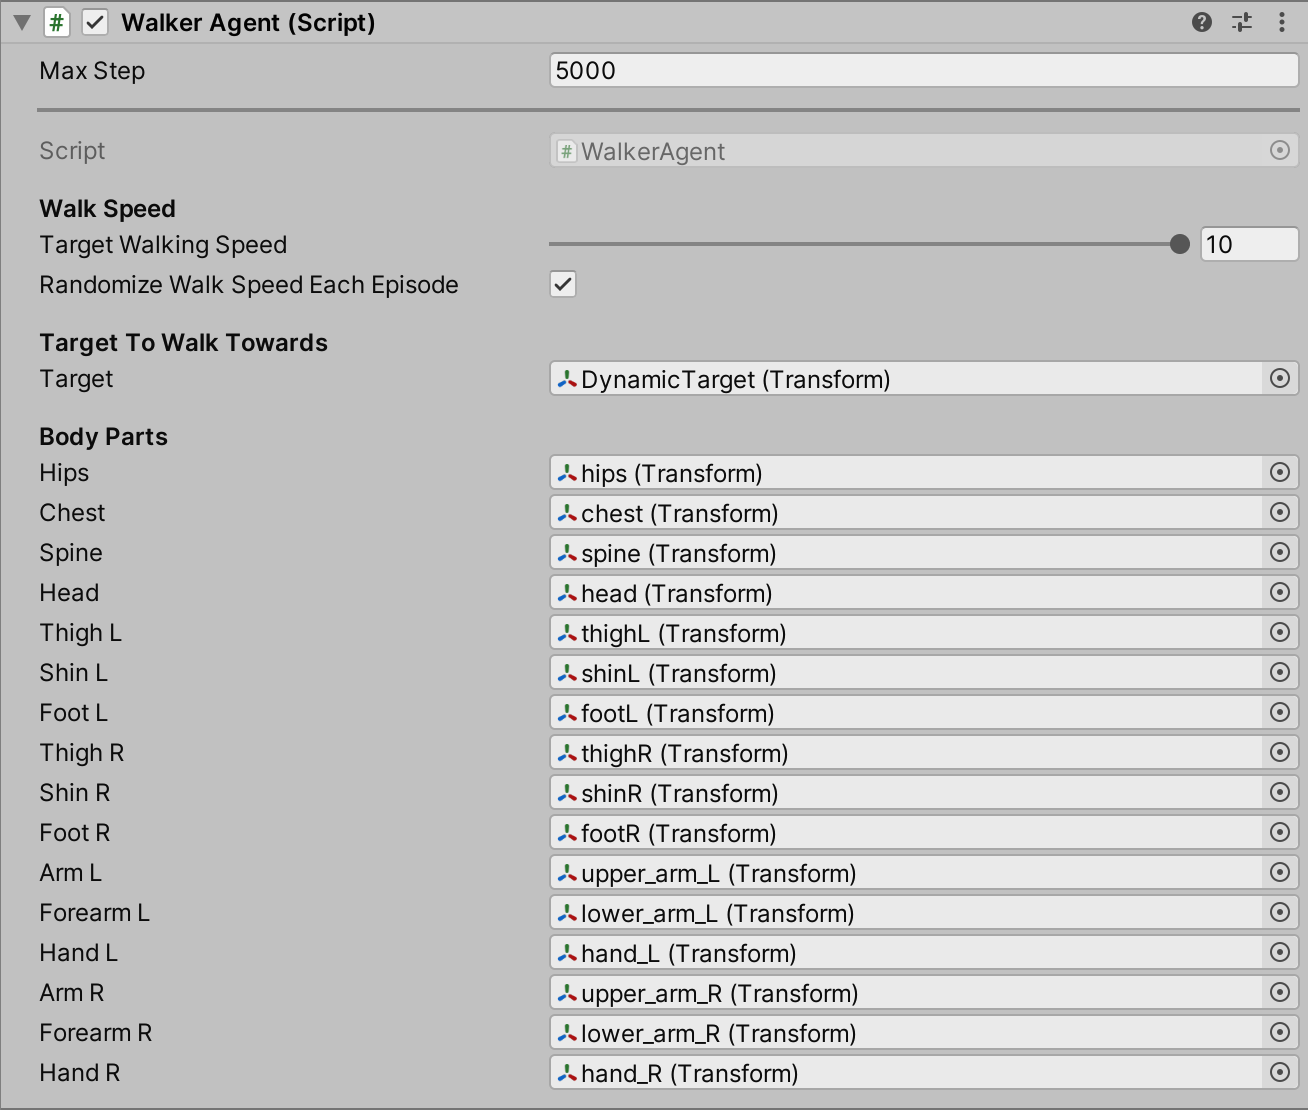
\includegraphics[width=0.8\textwidth]{img/komponente_walker_agent}
  \caption{Agent Konfiguration}
  \label{fig:komponente_walker_agent}
\end{figure}

\section{Training}

Zu beginn werden die Körperteile in der Gelenk-Motor-Steuerung initialisiert und das Ziel auf eine zufällige Position gesetzt.
Darauf folgend beginnt die Simulation der Trainingsepisoden. Hierfür werden alle Körperteile in ihre Startposition und die Rotation des Läufers um die Y Achse zufällig gesetzt. Die zufällige Rotation hilft dabei, das Verhalten des Läufers flexibel zu gestalten. Es wird weiterhin eine zufällige Zielgeschwindigkeit gewählt, um zusätzliche Stabilität zu gewährleisten.

Sind die Vorbereitungen getroffen, beginnt die Simulation mit einer Updatefrequenz von 75 Hz für die Phsikkalkulation. Der Agent fragt jedes fünfte Physikupdate eine Entscheidung an. Bei der Simulationsfrequenz von 75 Hz ergibt das eine Frequenz von 15 Anfragen pro Sekunde. Der Grund dafür, das die Anfragen nur jedes fünfte Update angefragt werden ist, dass der Agent durch diese Einschränkung seine Bewegungen genauer wählen muss. Es kann so verhindert werden, dass der Agent zu hastige und ruckartige Bewegungswechsel lernt. Sobald eine Entscheidung angefragt ist, erfasst der Agent den Zustand der Umgebung. Dieser wird anschließend im referenzierten Verhalten ausgewertet und eine Aktion ausgewählt.

Die Beobachtung des Agenten wird in Tabelle \ref{table:walker_beobachtung} dargestellt. Für jedes Körperteil wird die Beobachtung aus Tabelle \ref{table:walker_beobachtung_körperteil} dem Zustand angefügt. Die Beobachtungen müssen den Zustand des Läufers und der Umgebung im Bezug auf das Trainingsziel genau darstellen. Nur so kann der Agent die Situation verstehen, eine passende Aktion auswählen und gleichermaßen sein Verhalten optimieren. Um die Positionen und Rotationen der Körperteile mit möglichst wenig Ablenkung einzufangen, wird ein Stabilisierungsobjekt verwendet. Das Stabilisierungsobjekt wird in jedem Physikupdate auf die neue Hüftposition gesetzt. Die Richtung wird zusätzlich von der Hüfte in Richtung Ziel festgelegt. Die Verwendung dieses Stabilisierungsobjektes hat zur Folge das alle Bewegungen relativ zu einer gemeinsamen Basis abgebildet werden. Koordinaten unterschiede spielen dadurch keine Rolle. Der Läufer kann ein einziges Verhalten in Zielrichtung erlernen.\hl{korrektur lesen}

\begin{table}[H]
  \centering
  {\rowcolors{1}{gray!10}{white}
  \begin{tabular}{ |p{1cm}|p{9cm}|p{5cm}|}
  \hline
  \textbf{ID} & \textbf{Beobachtung} & \textbf{Anmerkung}  \\
  \hline
  \rowids & Abweichung Durchschnittsgeschwindigkeit von Zielgeschwindigkeit &  \\
  \hline
  \rowids & Durchschnittsgeschwindigkeit &  \\
  \hline
  \rowids & Zielgeschwindigkeit & \\
  \hline
  \rowids & Abweichung Hüftrotation von Zielrotation & \\
  \hline
  \rowids & Abweichung Kopfrotation von Zielrotation & \\
  \hline
  \rowids & Zielposition & \\
  \hline
  \rowids & Körperteil Beobachtungen & Beobachtung aus Tabelle \ref{table:walker_beobachtung_körperteil} für jedes Körperteil \\
  \hline
  \end{tabular}}
  \caption{Walker Agent Beobachtung}
  \label{table:walker_beobachtung}
\end{table}
\rowidsclear

\begin{table}[H]
  \centering
  {\rowcolors{1}{gray!10}{white}
  \begin{tabular}{ |p{1cm}|p{9cm}|p{5cm}|}
  \hline
  \textbf{ID} & \textbf{Beobachtung} & \textbf{Anmerkung}  \\
  \hline
  \rowids & Bodenkontakt & \\
  \hline
  \rowids & Geschwindigkeit & \\
  \hline
  \rowids & Rotationsgeschwindigkeit & \\
  \hline
  \rowids & Position relativ zur Hüfte & \\
  \hline
  \rowids & LokaleRotation & Fehlt für Hüfte und Hände \\
  \hline
  \rowids & Gelenkstärke & Fehlt für Hüfte und Hände \\
  \hline
  \end{tabular}}
  \caption{Walker Agent Körperteil Beobachtung}
  \label{table:walker_beobachtung_körperteil}
\end{table}
\rowidsclear

Das Format einer Aktion besteht aus den in Tabelle \ref{table:walker_aktion} aufgeführten Feldern für jedes Körperteil des Läufers, ausgenommen der Hüfte und Hände. Jedes Körperteil wird somit separat bewegt, um die Bewegungen zu optimieren und schlussendlich das Gleichgewicht zu halten und das Fortbewegen zu erlernen.

Die Hüfte ist das zentrale Körperteil, woran alle weiteren Körperteile mit Gelenken direkt oder indirekt anknüpfen. Aufgrund dieser zentralen Rolle wird die Hüftbeugung über das Gelenk des verbundenen Körpers gesteuert.

Da die Hände kaum Relevanz für das laufen haben, sind sie in der Demo fest mit dem Unterarm verbunden und brauchen daher nicht gesteuert werden.

\begin{table}[H]
  \centering
  {\rowcolors{1}{gray!10}{white}
  \begin{tabular}{ |p{1cm}|p{9cm}|p{5cm}|}
  \hline
  \textbf{ID} & \textbf{Beobachtung} & \textbf{Anmerkung}  \\
  \hline
  \rowids & Rotationswinkel X & Nur wenn Körperteil X Rotation beweglich ist\\
  \hline
  \rowids & Rotationswinkel Y & Nur wenn Körperteil Y Rotation beweglich ist\\
  \hline
  \rowids & Rotationswinkel Z & Nur wenn Körperteil Z Rotation beweglich ist\\
  \hline
  \rowids & Gelenkstärke & \\
  \hline
  \end{tabular}}
  \caption{Walker Agent Aktion}
  \label{table:walker_aktion}
\end{table}
\rowidsclear

Nach dem Erhalten der Aktion werden über die Gelenk-Motor-Steuerung die Zielrotationen, sowie die maximale Kraft des Gelenks festgelegt, und somit der Läufer gesteuert.

Die Belohnungsfunktion enthält zwei Komponenten. Zum einen wird die Differenz der Bewegung in Zielrichtung zwischen momentaner Bewegung und Zielbewegung durch die Funktion $R_V$ (abgebildet in \ref{fig:plot_demo_vel_1}) bewertet. Somit wird der Läufer dazu motiviert, effizient auf das Ziel zuzusteuern, indem Geschwindigkeit und Richtung optimiert werden. Zum Anderen wird die Abweichung zwischen momentaner Blickrichtung und der Zielrichtung in $R_L$ (abgebildet in \ref{fig:plot_demo_look}) bewertet. Diese Komponente stellt sicher, dass der Läufer sich vorwärts geradeaus auf das Ziel bewegt. Die Belohnung ergibt sich am Ende durch die Multiplikation beider Teilterme. Die Verwendung der Multiplikation hat zur Folge, dass die Belohnung gleichermaßen von beiden Teiltermen abhängig ist und es somit notwendig ist, beide Teile gleichzeitig zu optimieren. Als Ergebnis lernt der Läufer gleichermaßen die Ausrichtung als auch die Bewegung in Zielrichtung.

\begin{figure}[H]
  \centering  
  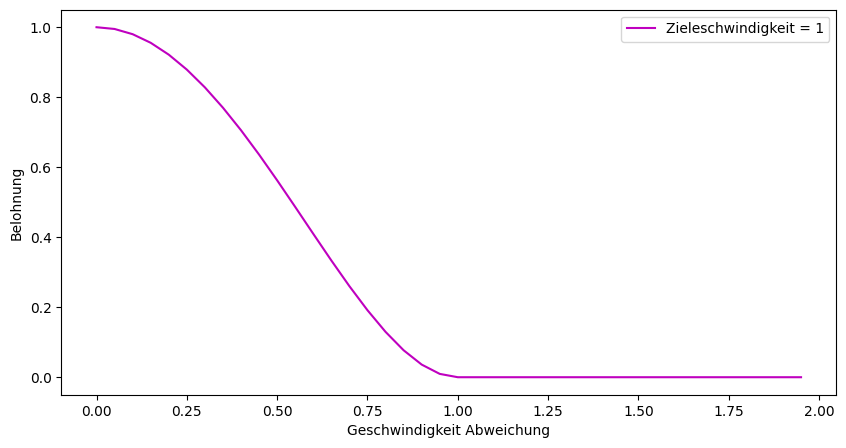
\includegraphics[width=0.9\textwidth]{img/plot_demo_vel_1}
  \caption{Walker Demo Match Velocity Belohnungsfunktion}
  \label{fig:plot_demo_vel_1}
\end{figure}

\begin{figure}[H]
  \centering  
  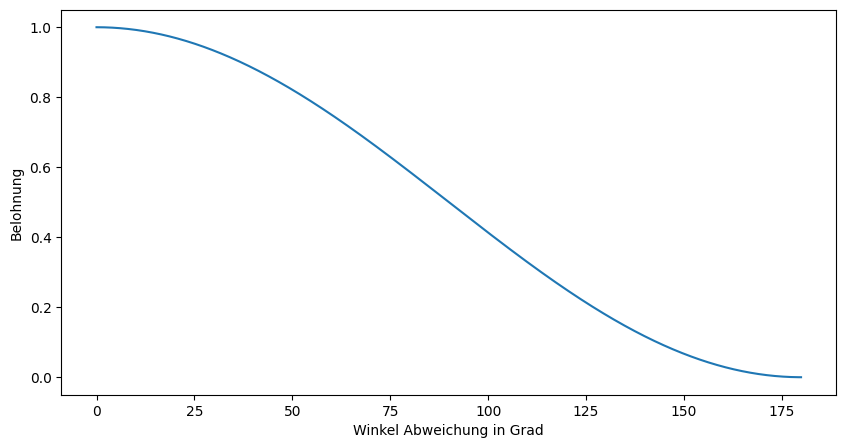
\includegraphics[width=0.9\textwidth]{img/plot_demo_look}
  \caption{Walker Demo Look At Target Belohnungsfunktion}
  \label{fig:plot_demo_look}
\end{figure}

Die Belohnung wird in jedem Physikupdate neu berechnet und dem Agenten hinzugefügt. Die Belohnung wird für den Zeitraum zwischen zwei Entscheidungen aufsummiert. Bevor die nächste Entscheidung getroffen wird, wird das Tupel aus Beobachtung, Aktion und erhaltener Belohnung im Trainingspuffer gespeichert. Hat der Puffer genug Informationen gespeichert, beginnt ein Lernprozess, in welchem die zuvor gespeicherten Tupel evaluiert werden. Es wird der PPO Algorithmus auf Teilbatches ausgeführt und so schrittweise das Verhalten angepasst.

Erreicht der Läufer ein Ziel, wird dieses an eine neue zufällige Position in der Umgebung bewegt.

Die Trainingsepisode läuft solange, bis entweder 5000 Schritte erreicht sind oder der Läufer fällt. Wenn ein Körperteil des Läufers, ausgenommen den Füßen und Schienbeinen, den Boden berührt, wird die Trainingsepisode sofort beendet. Diese Technik nennt man \grqq{}frühes Stoppen\grqq{}. Fällt der Läufer, benötigt es eine sehr komplexe Reihenfolge an Aktionen, um zurück auf die Beine zu kommen. Das frühe Stoppen ermöglicht dem Läufer, weniger Zeit für das Lernen irrelevanter Bewegungsabläufe zu verlieren. Ist die Episode zu Ende, wird sofort eine neue gestartet.

\section{Auswertung}
Unity stellt für die Demonstrationen Konfigurationsdateien für alle unterstützten Lernalgorithmen bereit. Unity ML-Agents implementiert sowohl PPO als auch SAC. Beide Algorithmen werden erfolgreich für die Verwendung bei kontinuierlichen Kontrollproblemen, wie dem in dieser Arbeit thematisierten Kontrollproblem eines zweibeinigen Charakters, eingesetzt. Ein großes Aushängeschild des SAC-Algorithmus ist seine Sample-Effizienz, was bedeutet, dass mit weniger Simulationsschritten ein besseres Ergebnis erzielt wird. Bei ersten Versuchen mit der Walker-Demo ist dies auch zu beobachten. Jedoch zeigt sich, dass trotz der unterschiedlichen Anzahl an Simulationsschritten die verbrachte Zeit, um ein Ergebnis zu erreichen, vergleichbar ist. Dies deutet darauf hin, dass der SAC-Algorithmus zwar effizienter mit den verfügbaren Daten umgeht, aber nicht zwangsläufig schneller zu einem brauchbaren Ergebnis führt. Ein Nachteil dieser Effizienz ist, dass durch die geringere Anzahl an Simulationsschritten auch weniger Daten erfasst werden, was zu weniger aufschlussreichen Auswertungen führt. Zudem zeigte sich in den ersten Tests, dass der PPO-Algorithmus zu einem natürlicheren Verhalten des Charakters führt. Aus diesen Gründen wird in folgenden Kapiteln der ppo Algorithmus zur Entwicklung verwendet.\hl{korrektur lesen}

Der Agent der Walker Demo erlernt im Laufe von 30 Millionen Trainingsschritten ein Verhalten, welches beinahe die Grenze der Episodenlänge erreicht, ohne zu fallen. In Abbildung \ref{fig:116_episode_length} wird die durchschnittlich erreichte Episodenlänge in Anfragen pro Episode dargestellt. Mit 800 Anfragen pro Episode kommt man auf 4000 Trainingsschritte beziehungsweise Physikupdates. Dabei erreicht er eine durchschnittliche Belohnung pro Episode von 1600 (siehe Abbildung \ref{fig:116_cumulative_reward}). Die durchschnittliche Belohnung ist ohne Kontext erstmal nur eine Zahl. Schaut man jedoch genauer, ergibt sich die durchschnittliche Belohnung aus der durchschnittlichen Episodenlänge und der durchschnittlich erreichten Belohnung. Teilt man die durchschnittliche Belohnung mit der Anzahl an Schritten, kommt man auf eine durchschnittliche Belohnung von ca. 0.4 pro Schritt. Die im Verlauf der Arbeit hinzugefügten Statistiken der Belohnungen zeigen eine Aufteilung von 0.9 Belohnung für die Blickrichtung und 0.45 für das Halten der Zielgeschwindigkeit (siehe Abbildung \ref{fig:116_look_reward}, \ref{fig:116_vel_reward}). Eine Blickrichtungsbelohnung von 0.9 ergibt eine Abweichung von durchschnittlich 35 Grad. Die Zielgeschwindigkeitsbelohnung ergibt eine Abweichung von ca. 51\%.

\begin{figure}[H]
  \centering
    \begin{subfigure}{.49\textwidth}
      \centering  
      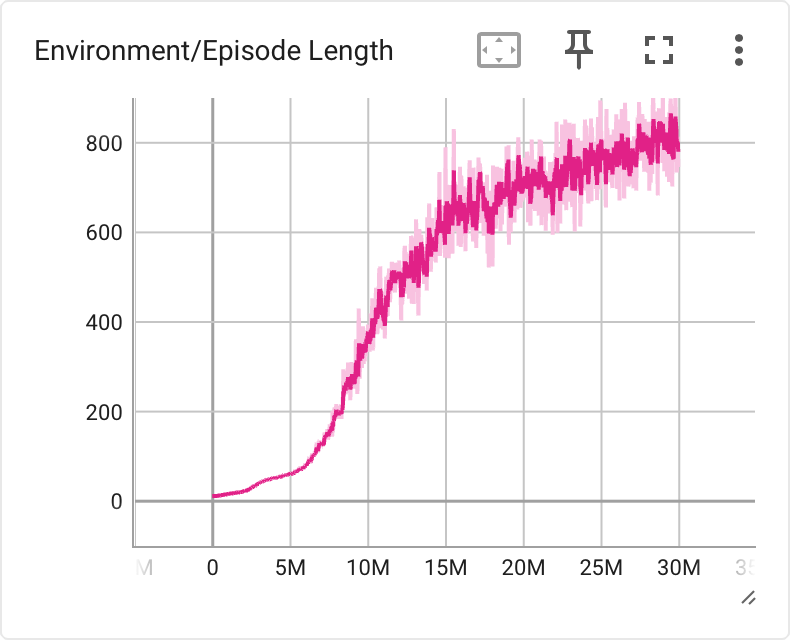
\includegraphics[width=\textwidth]{img/116_episode_length}
      \caption{Episodenlänge}
      \label{fig:116_episode_length}
    \end{subfigure}
    \begin{subfigure}{.49\textwidth}
      \centering  
      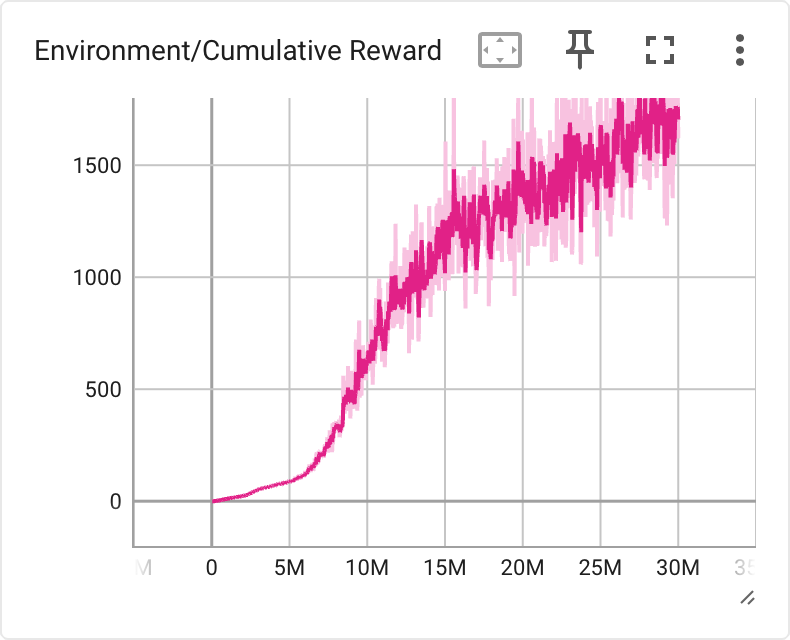
\includegraphics[width=\textwidth]{img/116_cumulative_reward}
      \caption{Angehäufte Belohnung}
      \label{fig:116_cumulative_reward}
    \end{subfigure}
     \begin{subfigure}{.49\textwidth}
      \centering  
      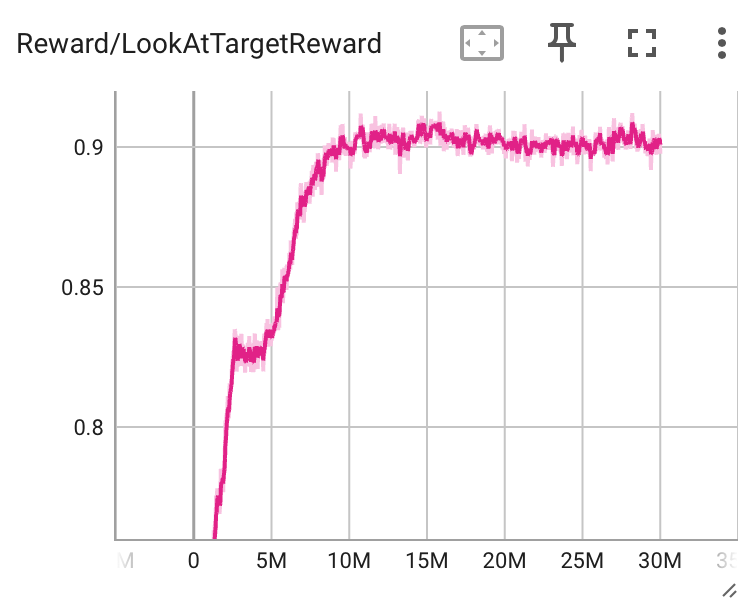
\includegraphics[width=\textwidth]{img/116_look_reward}
      \caption{Blickbelohnung}
      \label{fig:116_look_reward}
    \end{subfigure}
    \begin{subfigure}{.49\textwidth}
      \centering  
      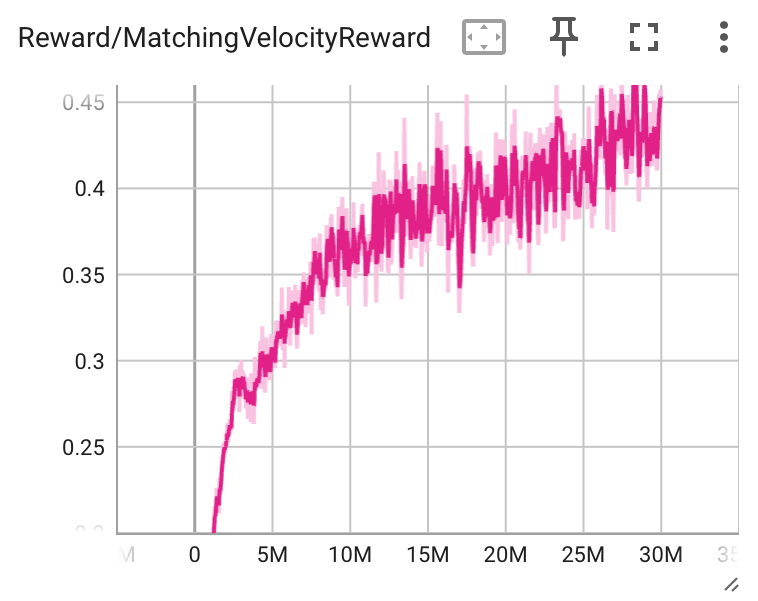
\includegraphics[width=\textwidth]{img/116_vel_reward}
      \caption{Geschwindigkeitsbelohnung}
      \label{fig:116_vel_reward}
    \end{subfigure}
    \begin{subfigure}{.49\textwidth}
      \centering  
      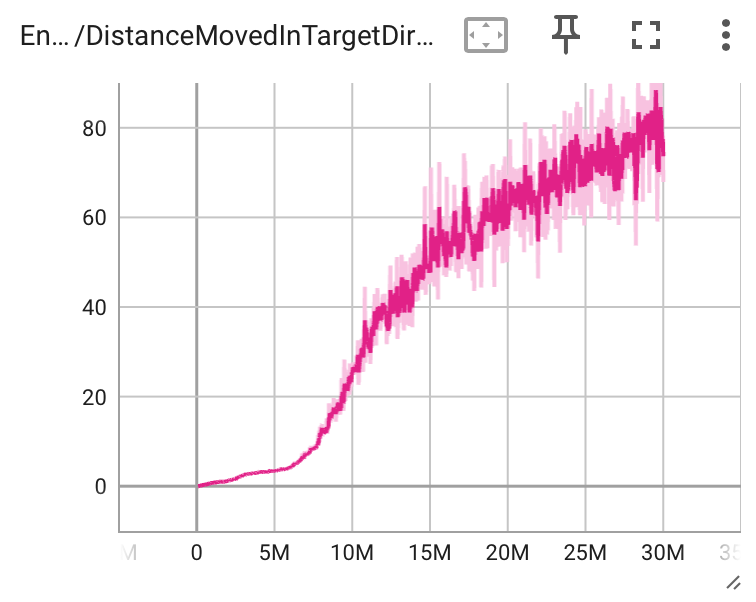
\includegraphics[width=\textwidth]{img/116_move_target_dir}
      \caption{Zurückgelegte Stecke in Zielrichtung}
      \label{fig:116_move_target_dir}
    \end{subfigure}
    \begin{subfigure}{.49\textwidth}
      \centering  
      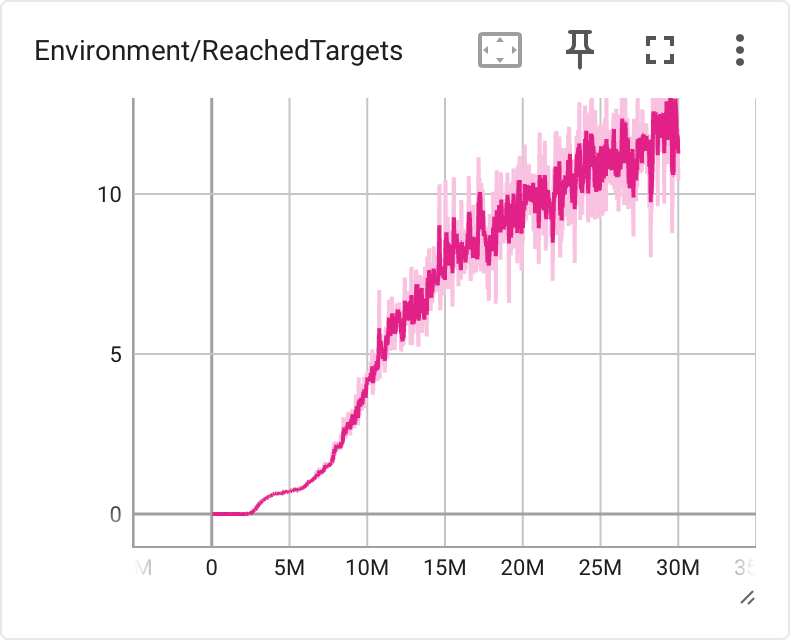
\includegraphics[width=\textwidth]{img/116_reach_target}
      \caption{Anzahl erreichte Ziele}
      \label{fig:116_reach_target}
    \end{subfigure}
    \caption{Walker Demo Training Graphen}
      \label{fig:116_training_graph}
\end{figure}

Der Läufer ist nicht in der Lage, die Belohnungen pro Zeitschritt maximal auszureizen, sondern steigert die Länge der Episode, indem er die Sturzrisiken minimiert. Dies führt zu steigender Belohnung innerhalb der Episode. Wie in Abbildung \ref{fig:116_move_target_dir} und \ref{fig:116_reach_target} zu sehen ist, läuft er während einer Episode durchschnittlich eine Distanz von 80 Einheiten und erreicht dabei 10,4 Ziele. Der Läufer lernt sich stabil zum Ziel zu bewegen. In Abbildung \ref{fig:analyse_gangbild} ist das Gangbild des Läufers abgebildet. Der Läufer wechselt periodisch das Standbein, setzt den einen Fuß vor den anderen und drückt sich über das Standbein voran. Durch die vereinfachte Darstellung der Füße kann der Läufer jedoch nicht richtig abrollen. Die Arme hält der Läufer nahezu horizontal und schwingt diese sehr stark um das Gleichgewicht halten zu können. Das Gangbild ist daher menschenähnlich, aber nicht detailliert genug um in realistischeren Anwendungsbereichen als natürliche Gehbewegung dargestellt zu werden.

\begin{figure}[H]
  \centering
  \begin{subfigure}{.3\textwidth}
    \centering
    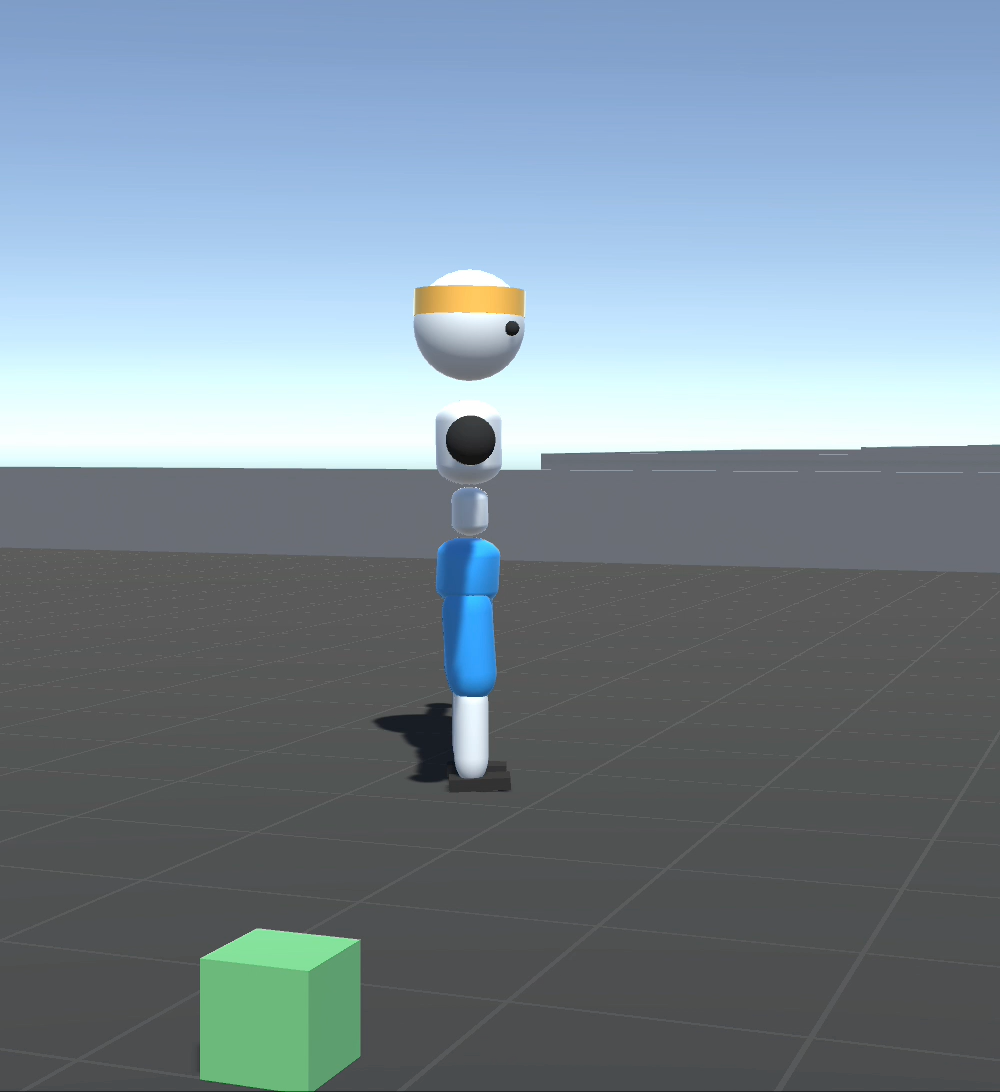
\includegraphics[width=\textwidth]{img/charakter_walker_1}
  \end{subfigure}
  \begin{subfigure}{.3\textwidth}
    \centering
    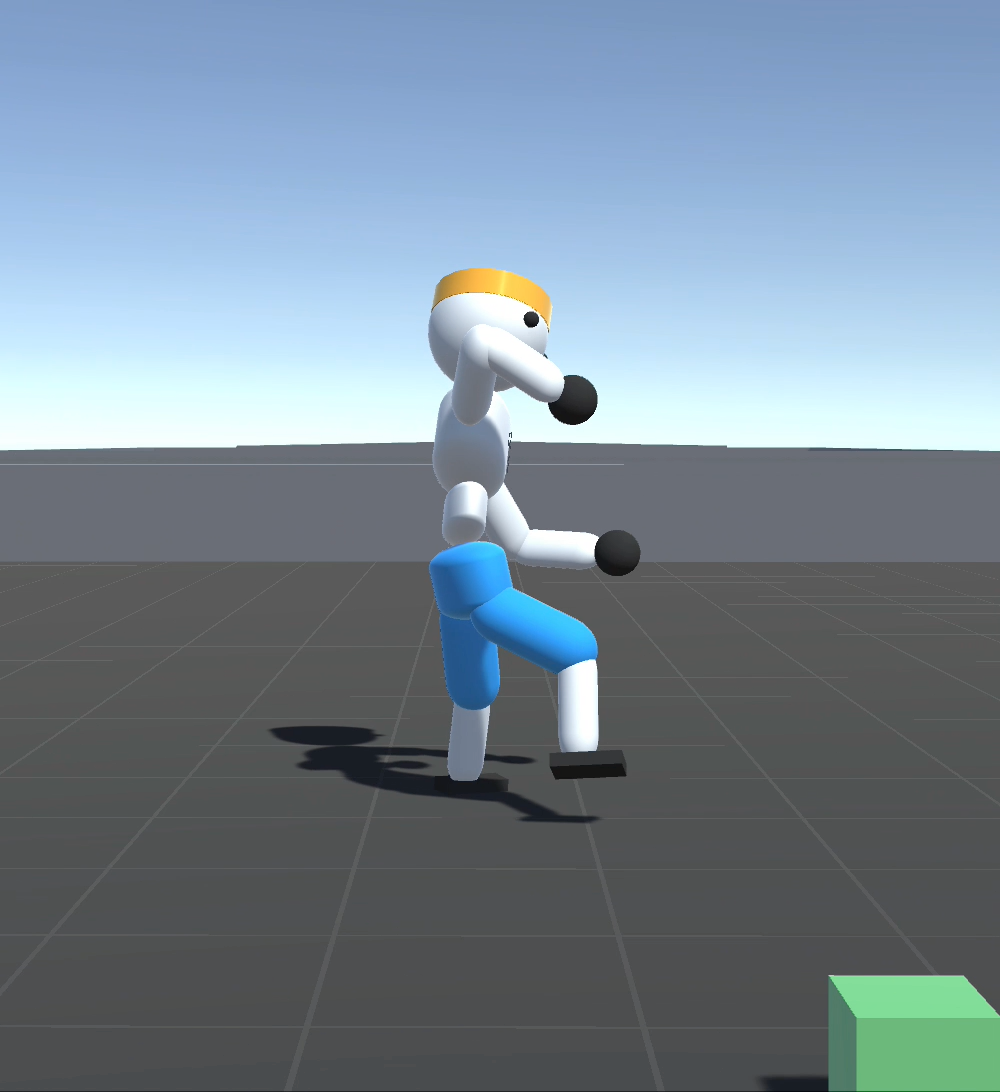
\includegraphics[width=\textwidth]{img/charakter_walker_2}
  \end{subfigure}
  \begin{subfigure}{.3\textwidth}
    \centering
    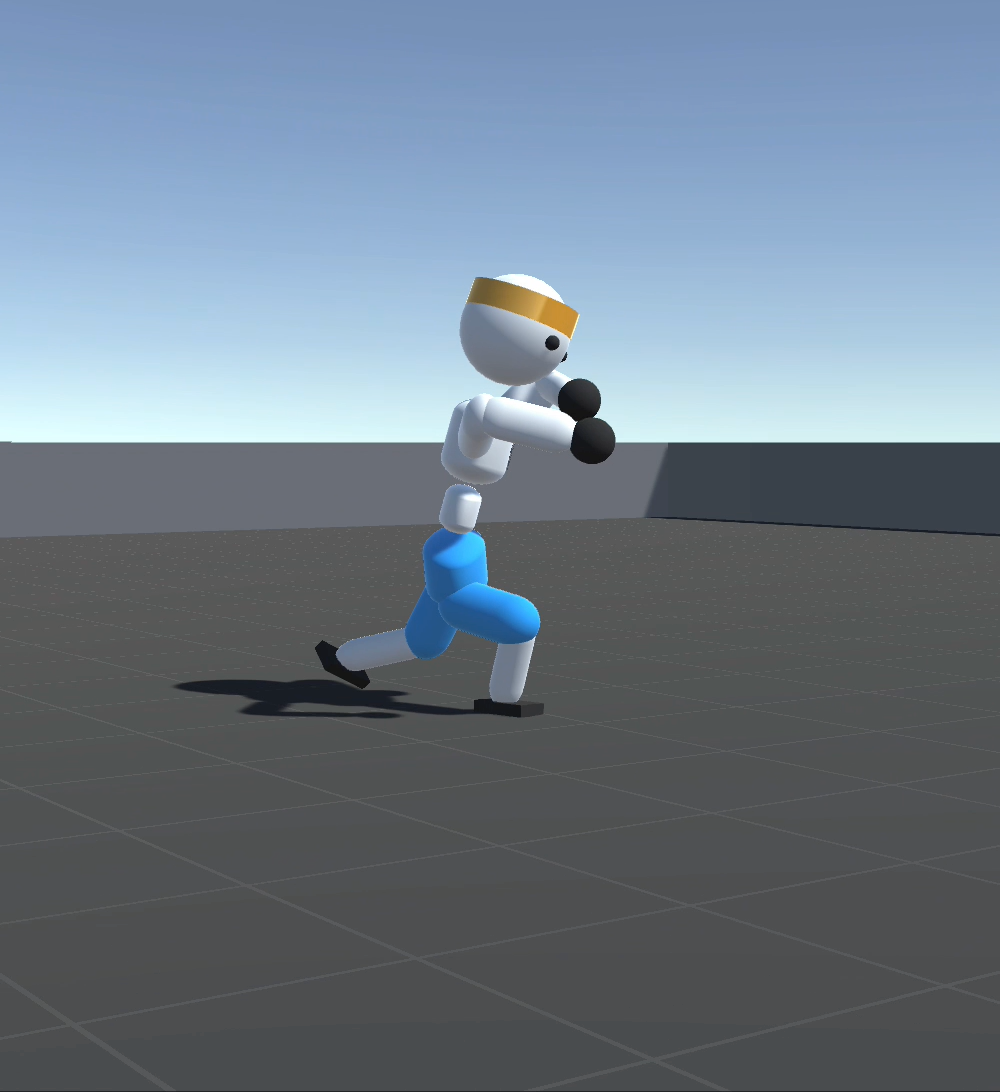
\includegraphics[width=\textwidth]{img/charakter_walker_3}
  \end{subfigure}
  \begin{subfigure}{.3\textwidth}
    \centering
    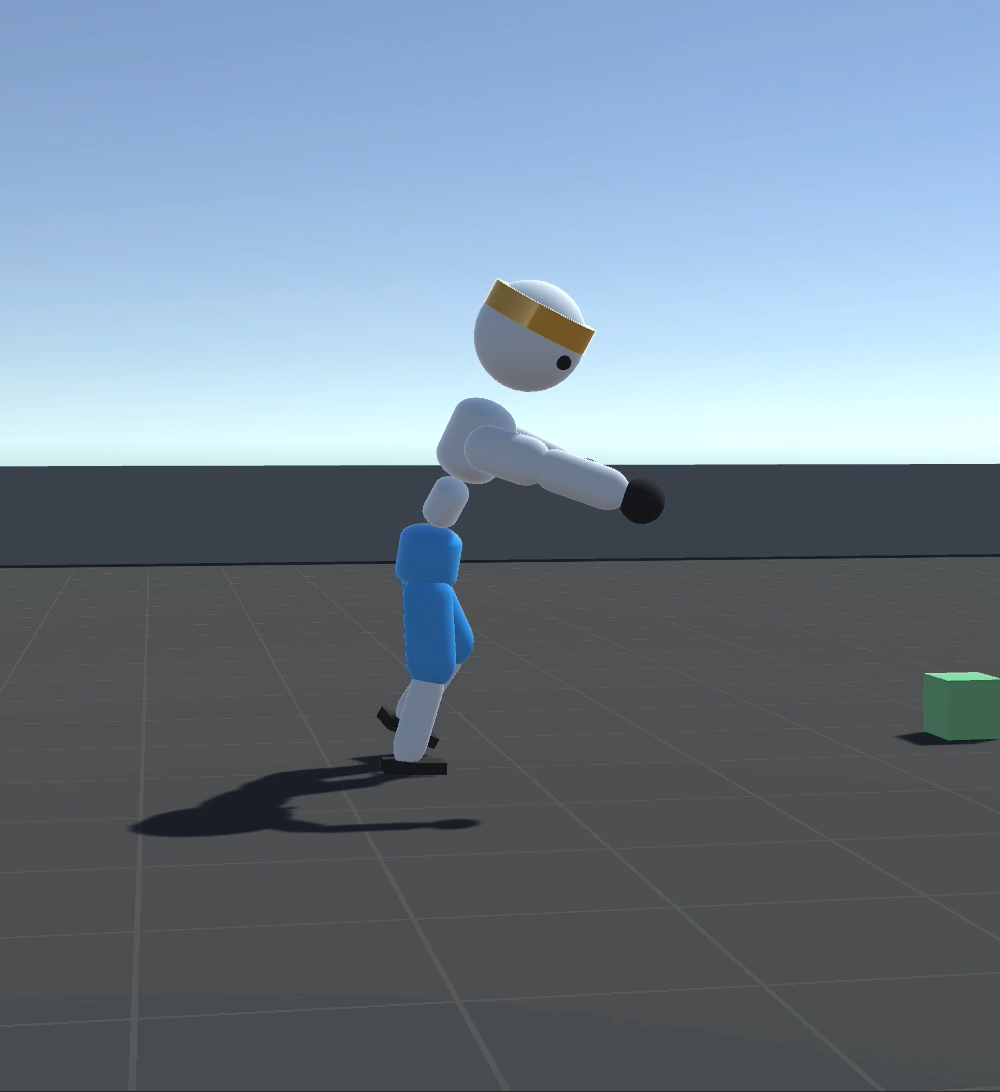
\includegraphics[width=\textwidth]{img/charakter_walker_4}
  \end{subfigure}
  \begin{subfigure}{.3\textwidth}
    \centering
    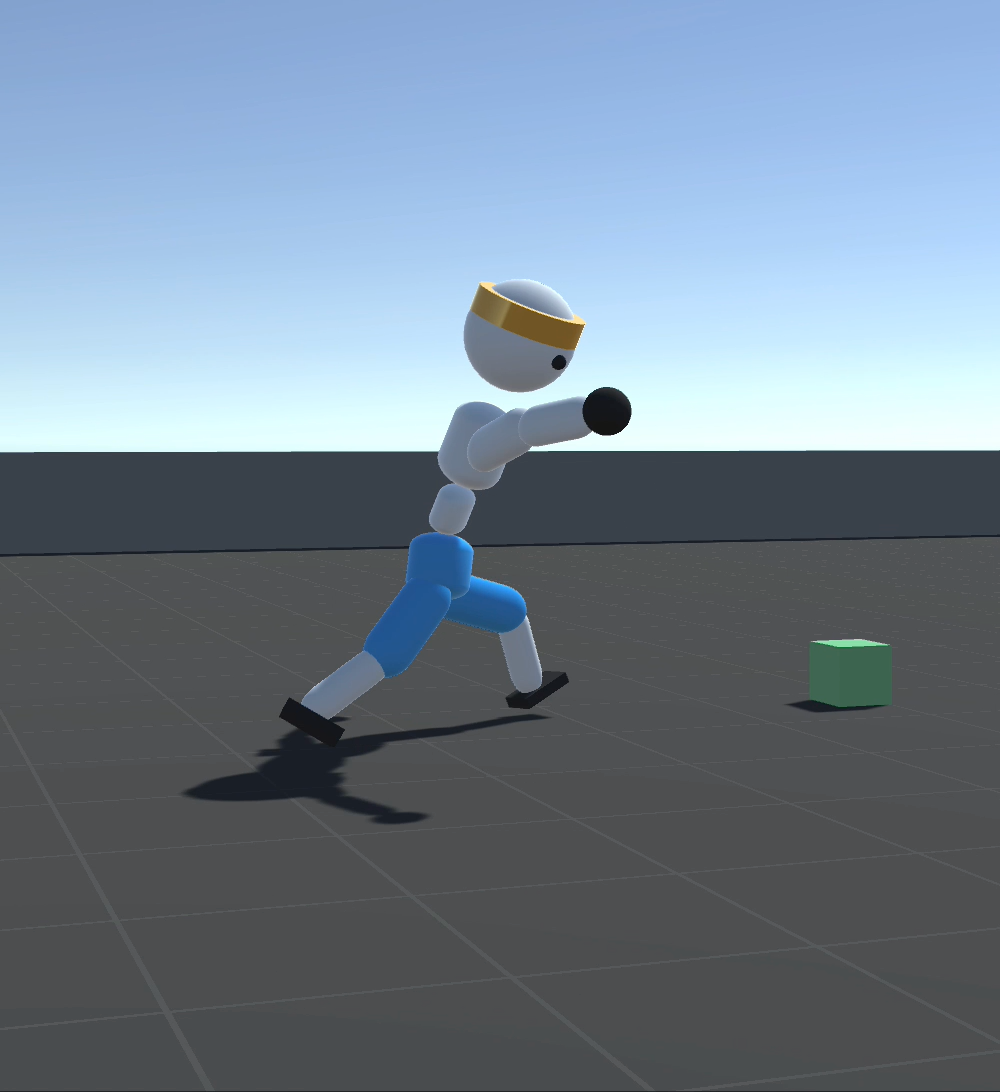
\includegraphics[width=\textwidth]{img/charakter_walker_5}
  \end{subfigure}
  \begin{subfigure}{.3\textwidth}
    \centering
    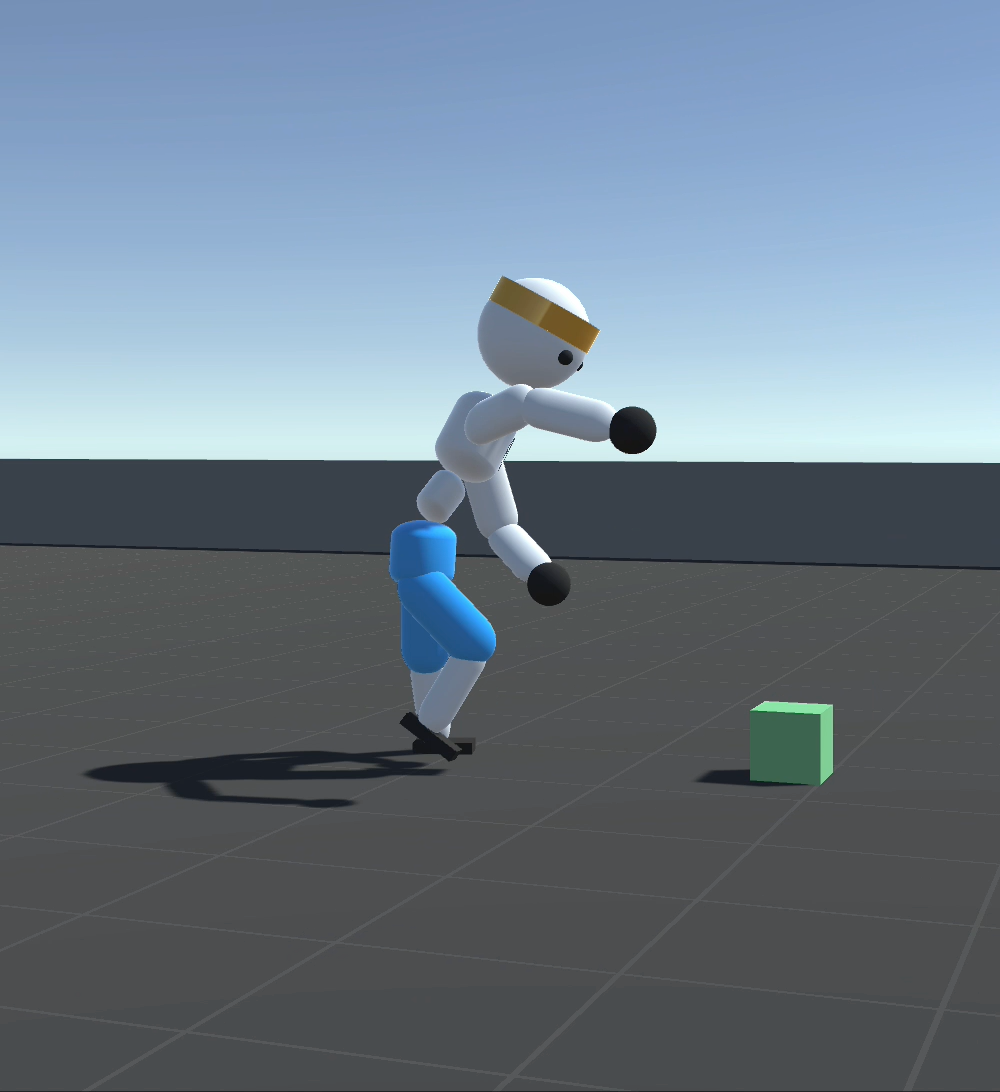
\includegraphics[width=\textwidth]{img/charakter_walker_6}
  \end{subfigure}
  \caption{Walker Demo Analyse Gangbild}
  \label{fig:analyse_gangbild}
\end{figure}
  